%% Section 1 of QM.tex (Quantum Mechanics Review). Compile QM.tex, not this file.
%% ============================================================
\section{Abstract Linear Space}
%% ============================================================

\paragraph{A vector space is a set closed under addition and scaling.} A \textcolor{blue}{vector space} $V$ is a set of objects, the vectors $|u\rangle$, $|v\rangle$, $|w\rangle$, that can be added and multiplied by numbers $a$, $b$. The first ten rules in Table~\ref{tab:axioms} define the vector space. The rules say nothing about lengths, angles or coordinates. A vector, therefore, exists on its own, like a stick lying on a table, before any ruler or coordinate system is chosen.

\begin{table}[h]
    \centering
    \caption{Rules of a vector space (first ten rows) and of an inner product (last three rows), for any vectors $|u\rangle$, $|v\rangle$, $|w\rangle$ in $V$ and any numbers $a$, $b$.}
    \label{tab:axioms}
    \renewcommand{\arraystretch}{1.3}
    \begin{tabular}{ll}
        \toprule
        Rule & Statement \\
        \midrule
        Closure under addition & $|u\rangle + |v\rangle \in V$ \\
        Commutative addition & $|u\rangle + |v\rangle = |v\rangle + |u\rangle$ \\
        Associative addition & $(|u\rangle + |v\rangle) + |w\rangle = |u\rangle + (|v\rangle + |w\rangle)$ \\
        Zero vector & $|u\rangle + 0 = |u\rangle$ \\
        Inverse & $|u\rangle + (-|u\rangle) = 0$ \\
        Closure under scalar multiplication & $a|u\rangle \in V$ \\
        Distributivity over vectors & $a(|u\rangle + |v\rangle) = a|u\rangle + a|v\rangle$ \\
        Distributivity over scalars & $(a+b)|u\rangle = a|u\rangle + b|u\rangle$ \\
        Associative scalar multiplication & $a(b|u\rangle) = (ab)|u\rangle$ \\
        Scalar identity & $1|u\rangle = |u\rangle$ \\
        \midrule
        Linearity of the inner product & $\langle w|\,(a|u\rangle + b|v\rangle) = a\langle w|u\rangle + b\langle w|v\rangle$ \\
        Conjugate symmetry & $\langle u|v\rangle = \langle v|u\rangle^*$ \\
        Positivity & $\langle u|u\rangle \geq 0$, with equality only for $|u\rangle = 0$ \\
        \bottomrule
    \end{tabular}
\end{table}

\paragraph{The inner product is the ruler that creates lengths and angles.} An \textcolor{blue}{inner product} is a rule that takes two vectors and returns one number, $\langle u | v \rangle$, and obeys the last three rules in Table~\ref{tab:axioms}. A complex vector space with an inner product is a \textcolor{blue}{Hilbert space}. The inner product is the metric of the space. The length of a vector and the angle $\theta$ between two real vectors follow from the inner product:
\begin{equation*}
    |u| = \sqrt{\langle u | u \rangle}, \qquad
    \cos\theta = \frac{\langle u | v \rangle}{|u|\, |v|}
\end{equation*}
The familiar form $|u|\, |v| \cos\theta$, therefore, cannot define the inner product, because the lengths and the angle already require the inner product. The three rules characterize every inner product but do not select one. A particular inner product is usually specified with one basis, by declaring that basis orthonormal. In the stick analogy, the inner product is the ruler, calibrated once with one basis. After the calibration, the length of the stick is fixed, and every other basis gives the same length. Only a different ruler, that is, a different inner product, gives a different length. The length is, therefore, fixed by the ruler, and the formula of the length in each basis adapts to reproduce the same length, not the other way around.

\paragraph{A basis turns a vector into a list of components.} A set $\{|e_i\rangle\}$ is an \textcolor{blue}{orthonormal basis} when every vector is a combination of the set and $\langle e_i | e_j \rangle = \delta_{ij}$. A vector is rebuilt from the components as
\begin{equation*}
    |v\rangle = \sum_i v_i\, |e_i\rangle, \qquad v_i = \langle e_i | v \rangle
\end{equation*}
The \textcolor{blue}{component} $v_i$ is a number. The projection of $|v\rangle$ onto $|e_i\rangle$ is the vector $|e_i\rangle\langle e_i | v \rangle = v_i\, |e_i\rangle$, not the number $v_i$. The fixed component $v_j$ follows from the orthonormality:
\begin{align*}
    \langle e_j | v \rangle &= \sum_i v_i\, \langle e_j | e_i \rangle \\
    &= \sum_i v_i\, \delta_{ji} \\
    &= v_j
\end{align*}
The summation index $i$ is a placeholder that runs over every basis vector, whereas $j$ selects one component. Substituting $v_i = \langle e_i | v \rangle$ back into the expansion gives $|v\rangle = \sum_i |e_i\rangle\langle e_i | v \rangle$ for every $|v\rangle$, which is the \textcolor{blue}{completeness relation}
\begin{equation*}
    \sum_i |e_i\rangle\langle e_i| = \mathbb{I}
\end{equation*}
The identity operator changes nothing, so inserting the completeness relation between a bra and a ket gives the inner product in terms of components:
\begin{align*}
    \langle u | v \rangle &= \sum_i \langle u | e_i \rangle \langle e_i | v \rangle \\
    &= \sum_i \langle e_i | u \rangle^{*} \langle e_i | v \rangle
\end{align*}
\begin{equation}
    \boxed{\langle u | v \rangle = \sum_i u_i^{*}\, v_i}
\end{equation}
The sum of products is the formula of the inner product in an orthonormal basis, not the definition of the inner product. Every orthonormal basis gives the same number, because every formula starts from the same $\langle u | v \rangle$.

\paragraph{A vector has no preferred basis.} Figure~\ref{fig:bases} shows two vectors $v$ and $w$ and two orthonormal bases, $\{e_1, e_2\}$ and $\{f_1, f_2\}$. Each basis is orthogonal within itself, but $f_1$ is not orthogonal to $e_1$ or $e_2$, and neither basis is singled out. The components of $v$ differ between the two bases, so $(v_1, v_2) \neq (v_1', v_2')$. The length of $v$ and the angle $\alpha$ between $v$ and $w$, however, are the same in both bases, because both quantities follow from the inner product alone. The basis does not set the length of a vector. A basis is needed only to write the vector as a list of numbers.

\begin{figure}[h]
    \centering
    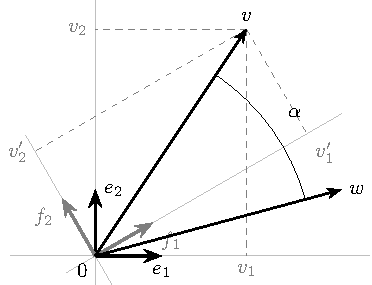
\includegraphics{two_bases.pdf}
    \caption{Two vectors $v$ and $w$ in two orthonormal bases, $\{e_1, e_2\}$ and the rotated basis $\{f_1, f_2\}$. The dashed lines project $v$ onto each basis vector. The components change from basis to basis, whereas the length of $v$ and the angle $\alpha$ do not.}
    \label{fig:bases}
\end{figure}

\paragraph{Orthogonality is defined by the inner product, not by the picture.} A right angle is the usual picture of orthogonality, but the picture already assumes the Euclidean inner product of the drawing plane. Two vectors are orthogonal when $\langle u | v \rangle = 0$, so a basis is orthonormal or skewed only with respect to a chosen inner product. The basis vectors $|g_1\rangle = (1, 0)$ and $|g_2\rangle = (-\tfrac{1}{2}, \tfrac{\sqrt{3}}{2})$, for example, are unit vectors at $120^\circ$ in the drawing plane. The Euclidean inner product of the two basis vectors is
\begin{equation*}
    \langle g_1 | g_2 \rangle = \cos 120^\circ = -\tfrac{1}{2}
\end{equation*}
The inner product is not zero, so the basis is not orthogonal under the Euclidean inner product. Written in its own coordinates, every basis looks like a set of unit columns, so $|g_1\rangle$ and $|g_2\rangle$ become $(1, 0)$ and $(0, 1)$. The sum of products of these columns is zero, but the sum-of-products formula assumes the orthonormality that is being tested, so the argument is circular. The same basis does become orthonormal under a new inner product, defined by $\langle g_i | g_j \rangle' = \delta_{ij}$ and extended linearly. Under the new inner product, however, the Euclidean axes $|\hat x\rangle = (1,0)$ and $|\hat y\rangle = (0,1)$ are no longer orthogonal. The axes expanded in the skewed basis are
\begin{equation*}
    |\hat x\rangle = |g_1\rangle, \qquad
    |\hat y\rangle = \tfrac{1}{\sqrt{3}}\,|g_1\rangle + \tfrac{2}{\sqrt{3}}\,|g_2\rangle
\end{equation*}
and the new inner product of the axes is
\begin{align*}
    \langle \hat x | \hat y \rangle' &= 1 \cdot \tfrac{1}{\sqrt{3}} + 0 \cdot \tfrac{2}{\sqrt{3}} \\
    &= \tfrac{1}{\sqrt{3}} \neq 0
\end{align*}
Each basis is, therefore, orthonormal under the inner product calibrated with that basis, and one inner product cannot make every basis orthonormal at the same time.

\paragraph{A rescaled basis changes the components, not the length.} The basis $|e_i'\rangle = 2|e_i\rangle$ is orthogonal but not normalized, with $\langle e_i' | e_j' \rangle = 4\,\delta_{ij}$. The same vector rewritten in the rescaled basis has half the components:
\begin{equation*}
    |v\rangle = \sum_i v_i\, |e_i\rangle = \sum_i \frac{v_i}{2}\, \bigl(2|e_i\rangle\bigr), \qquad v_i' = \frac{v_i}{2}
\end{equation*}
The squared length, computed with the inner products of the rescaled basis vectors, is unchanged:
\begin{align*}
    \langle v | v \rangle &= \sum_{i,j} v_i'^{*}\, v_j'\, \langle e_i' | e_j' \rangle \\
    &= 4 \sum_i |v_i'|^2 \\
    &= \sum_i |v_i|^2
\end{align*}
The sum of products $\sum_i |v_i'|^2$ would give one quarter of the squared length, because that formula holds only in an orthonormal basis. A rescaled basis and a skewed basis both fail to be orthonormal, the first because the basis vectors are not unit vectors and the second because the basis vectors are not orthogonal. In both cases the ruler fixes the length, and only the components and the formula change. Declaring $2|e_i\rangle$ to have unit length is a different ruler, which halves every length like a change of units.

\paragraph{The orthonormal bases of one inner product are linked by rotations and reflections.} Two orthonormal bases $\{|e_j\rangle\}$ and $\{|f_i\rangle\}$ under the same inner product are linked by a matrix $R$, with $|f_i\rangle = \sum_j R_{ji}\, |e_j\rangle$. The orthonormality of the new basis constrains $R$:
\begin{align*}
    \langle f_i | f_k \rangle &= \sum_{j,l} R_{ji}\, R_{lk}\, \langle e_j | e_l \rangle \\
    &= \sum_{j} R_{ji}\, R_{jk} \\
    &= (R^{T} R)_{ik}
\end{align*}
The condition $\langle f_i | f_k \rangle = \delta_{ik}$ then gives
\begin{equation}
    \boxed{R^{T} R = \mathbb{I}}
\end{equation}
A real matrix with $R^{T} R = \mathbb{I}$ is a rotation or a reflection, as in Fig.~\ref{fig:bases}. For complex coefficients, the transpose becomes the conjugate transpose, and the condition becomes $U^{\dagger} U = \mathbb{I}$ for a \textcolor{blue}{unitary} matrix $U$. Unitary transformations are, therefore, the complex version of rotations and reflections.

\paragraph{Summary of the misconceptions.} Table~\ref{tab:misconceptions} collects the misconceptions corrected in this section.

\begin{table}[h]
    \centering
    \caption{Common misconceptions about vectors, bases and inner products.}
    \label{tab:misconceptions}
    \renewcommand{\arraystretch}{1.3}
    \begin{tabular}{p{0.42\textwidth}p{0.48\textwidth}}
        \toprule
        Misconception & Correction \\
        \midrule
        The component $\langle e_i | v \rangle$ is the projection of $|v\rangle$. & The component is a number. The projection is the vector $|e_i\rangle\langle e_i | v \rangle$. \\
        The basis sets the length of a vector. & The inner product sets the length. Only the components depend on the basis. \\
        $|u|\,|v|\cos\theta$ defines the inner product. & The lengths and the angle are defined by the inner product, so the form is circular. \\
        Orthogonality means a right angle in the picture. & Orthogonality means $\langle u | v \rangle = 0$ under the chosen inner product. \\
        Every basis is orthonormal within itself, because the basis looks like unit columns in its own coordinates. & The sum-of-products formula assumes orthonormality, so the test is circular. \\
        The inner product is defined locally within each basis. & One inner product gives one number. The formulas in the bases are derived from it. \\
        Rescaling the basis by 2 halves the length. & Only the components halve. The formula picks up the factor $\langle e_i' | e_i' \rangle = 4$. \\
        \bottomrule
    \end{tabular}
\end{table}
